\chapter{Експериментальне дослідження чотирьохполюсників.} 
\label{chapter:first}

\section{Проба пера: дослідення перетворення прямокутних імпульсів}

Для отримання красивих картинок перетворення вхідного прямокутного сигналу очевидно був потрібний сам генератор сигналу. Оскільки розбиратися із версією, яка керується старичком ПК (який взагалі-то керується гордим Windows XP!) авторам було м'ягко кажучи лінь, було прийняте геніальне рішення - використати генератор DDS 9850, успішно апробований у \cite{lab3} та воскрешений у \cite{lab1}. Встановивши частоту $\omega = 10Hz$ та покрутивши трошки те, що крутити не треба було отримані красиві квадратні імпульси на вході та не менш красиві перетворені сигнали на виході \ref{fig:square}.

\begin{figure}[h]
	\begin{minipage}[h]{0.47\linewidth}
		\center{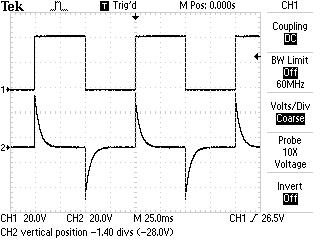
\includegraphics[width=1\linewidth]{square/D.png}} \\
	\end{minipage}
	\hfill
	\begin{minipage}[h]{0.47\linewidth}
		\center{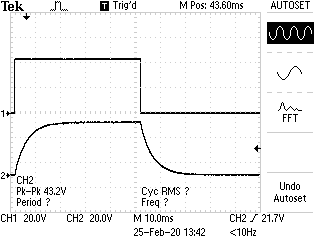
\includegraphics[width=1\linewidth]{square/I.png}} \\
	\end{minipage}
	\caption{Перетворення квадратних імпульсів для диферинціюючого та інтегруючого чотирьохполюсника}
	\label{fig:square}
\end{figure}

\section{Дослідження амплітудно-частотних та фазо-частотних характеристик приборів.}

Для виконання цього завдання ми подавали сигнал синусоїдальної форми різної частоти на вхід, та порівнювали з ним сигнал, що отримувався на виході з осцилографа. Здобуті надважким шляхом два набора точок у формі синусоїд \ref{fig:expsinI} та \ref{fig:expsinD} апроксимовувалися у програмі cern Root \cite{root}, а чисельні значення амплітуд та зсуву фаз порівнювалися, та записувалися відповідні значення $K(\omega)$ та $\phi(\omega)$. 

\begin{figure}[h]
	\center{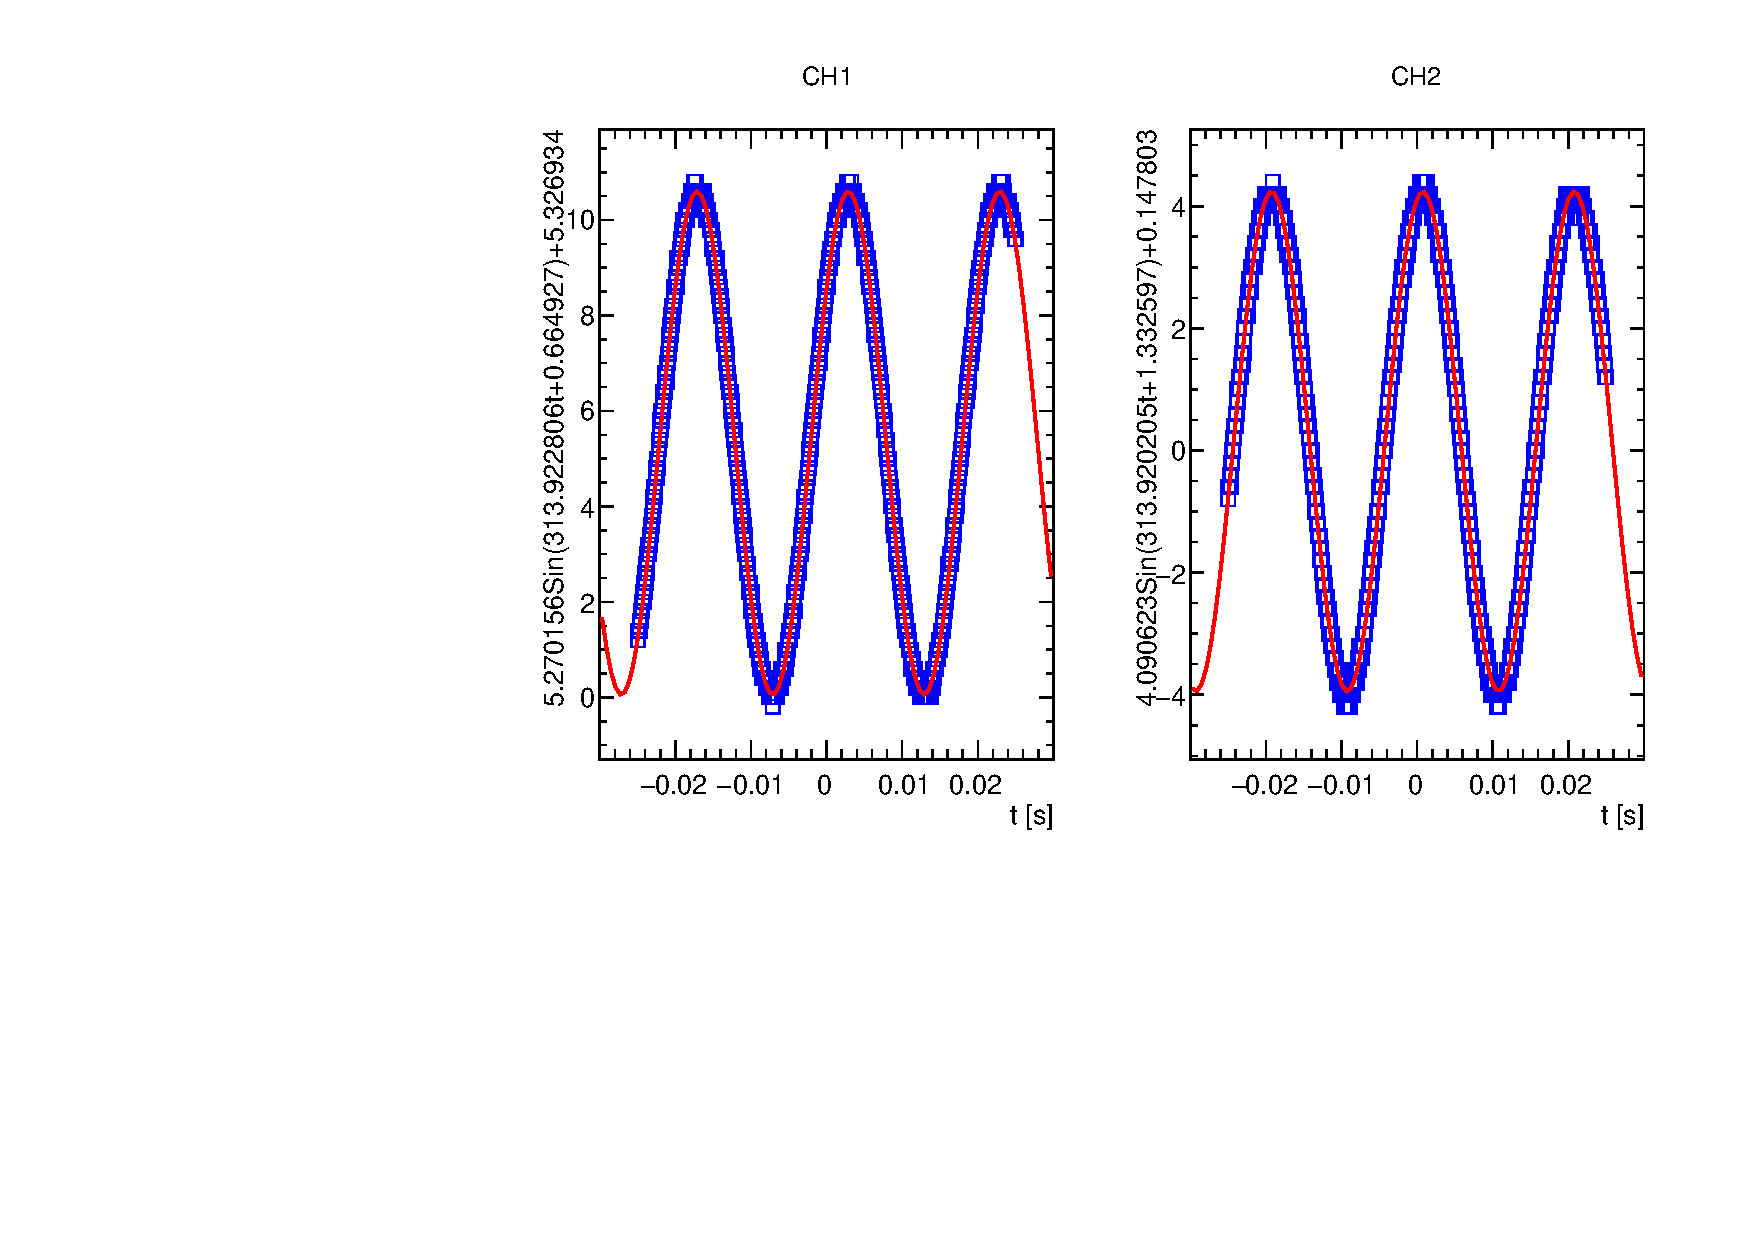
\includegraphics[width=1\linewidth,height=0.4\linewidth]{sind/sin.pdf}} \\
	\caption{Сигнал на вході (канал 1) та виході (канал 2) диферинціюйочого чотирьохполюсника при $\omega = 50Hz$. Параметри апроксимації написані у підписі до вертикальної осі.}
	\label{fig:expsinD}
\end{figure}

\begin{figure}[h]
	\center{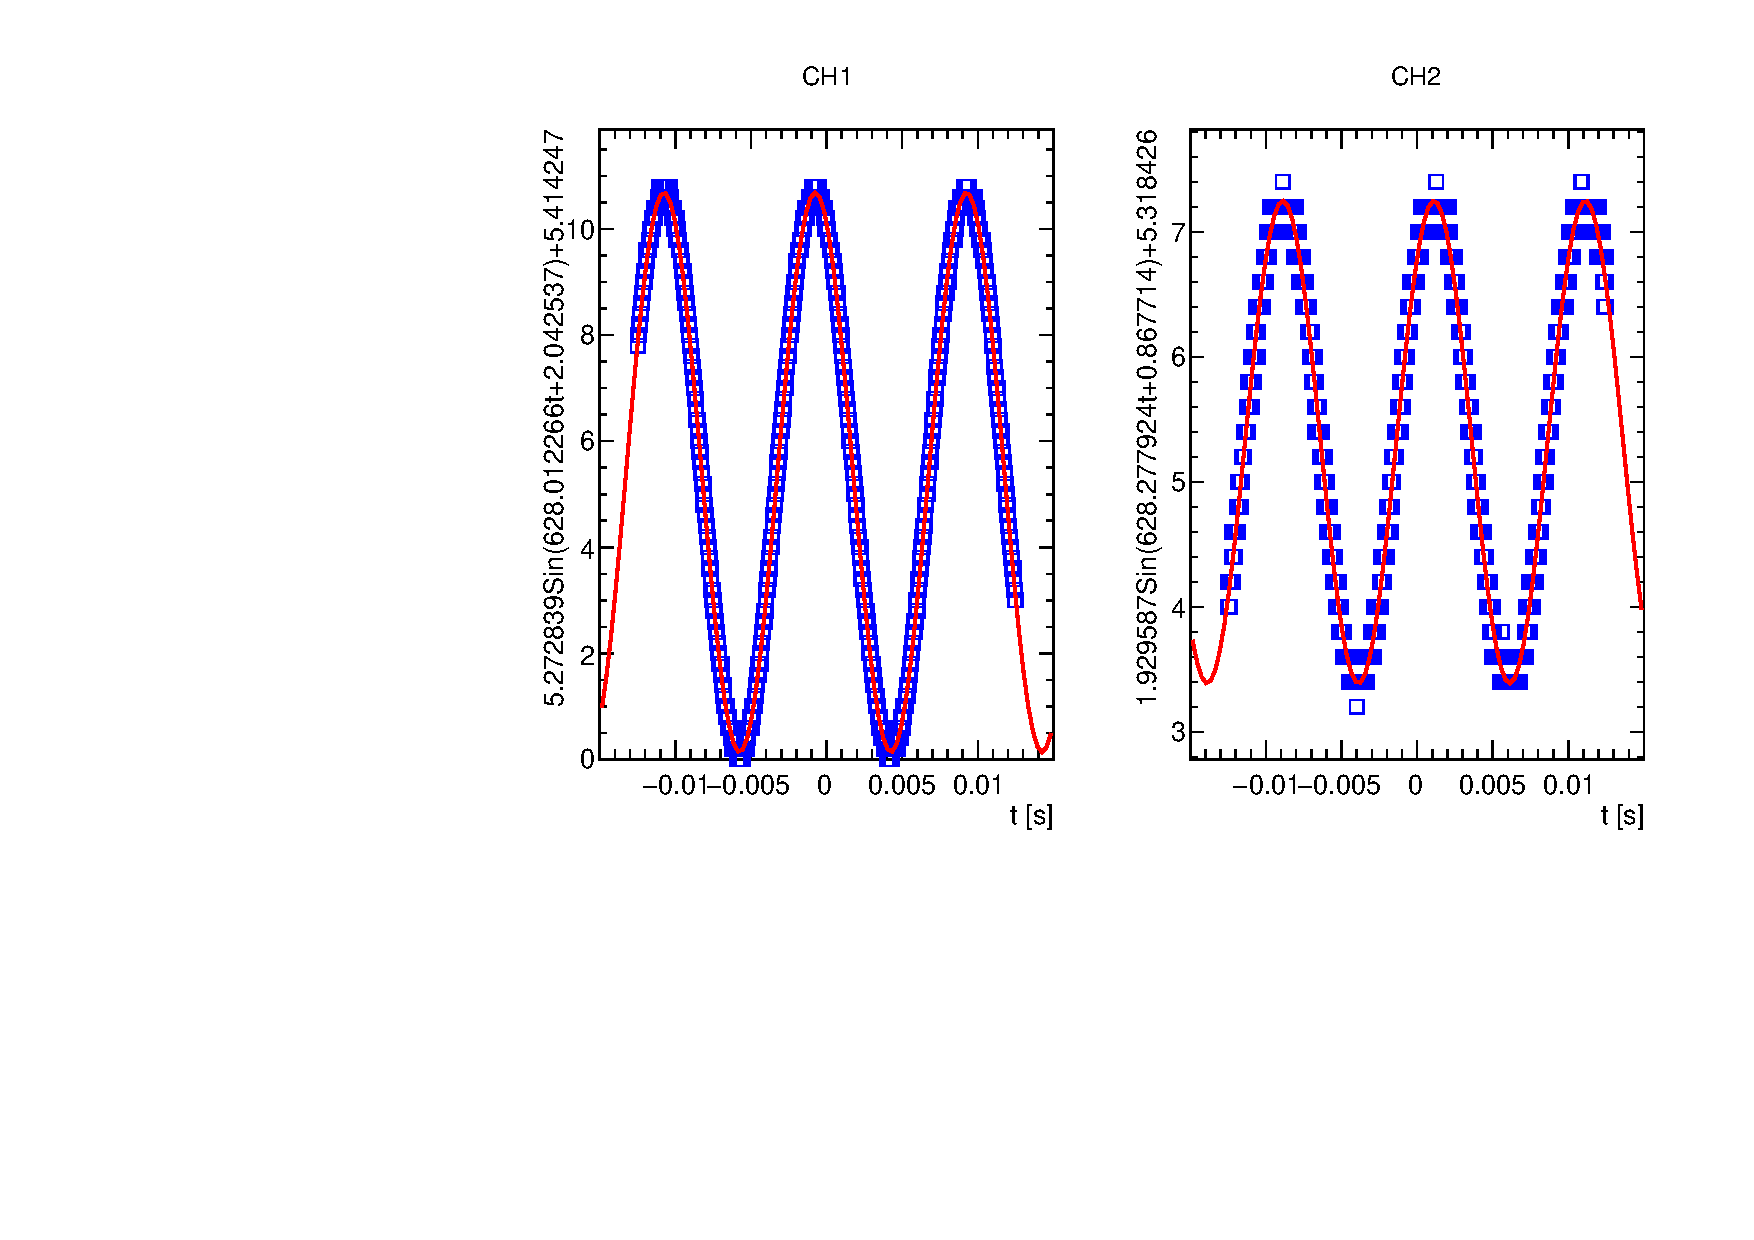
\includegraphics[width=1\linewidth,height=0.4\linewidth]{sini/sin.pdf}} \\
	\caption{Сигнал на вході (канал 1) та виході (канал 2) інтегруючого чотирьохполюсника при $\omega = 50Hz$. Параметри апроксимації написані у підписі до вертикальної осі.}
	\label{fig:expsinI}
\end{figure}

І таким чином ми отримували красиві графіки \ref{fig:expkph}. Звісно ми спробували апроксимувати ці точки за допомогою загальноприйнятих моделей \ref{theoryD} та \ref{theoryI} для диферинціюючих та інтегруючих чотирьохполюсників відповідно. 

\begin{equation}
	\begin{aligned}
		K = \frac{\omega RC}{\sqrt{1+(\omega R C)^2}}\\
		\phi = arctg(\frac{1}{\omega RC})
	\end{aligned}
	\label{theoryD}
\end{equation}

\begin{equation}
	\begin{aligned}
		K = \frac{1}{\sqrt{1+(\omega R C)^2}}\\
		\phi = -arctg(\omega RC)
	\end{aligned}
	\label{theoryI}
\end{equation}

Невідомим параметром при такій апроксимації виступає наглий добуток $RC$. Отримане значення (звісно за допомогою алгоритму MIGRAD/MINUIT) складало $RC = 4.0277 \pm  0.0383 ms$. 
Якщо тепер порахувати теоретичне значення даної величини ($R = 20k\Omega$, $C = 154nF$) отримаємо значення $RC = 3.08 ms$ - \textbf{от що робить паразитний опір та ємність з хорошими \sout{людьми} чотирьохполюсниками.}

\begin{figure}[h]
	\begin{minipage}[h]{0.4\linewidth}
		\center{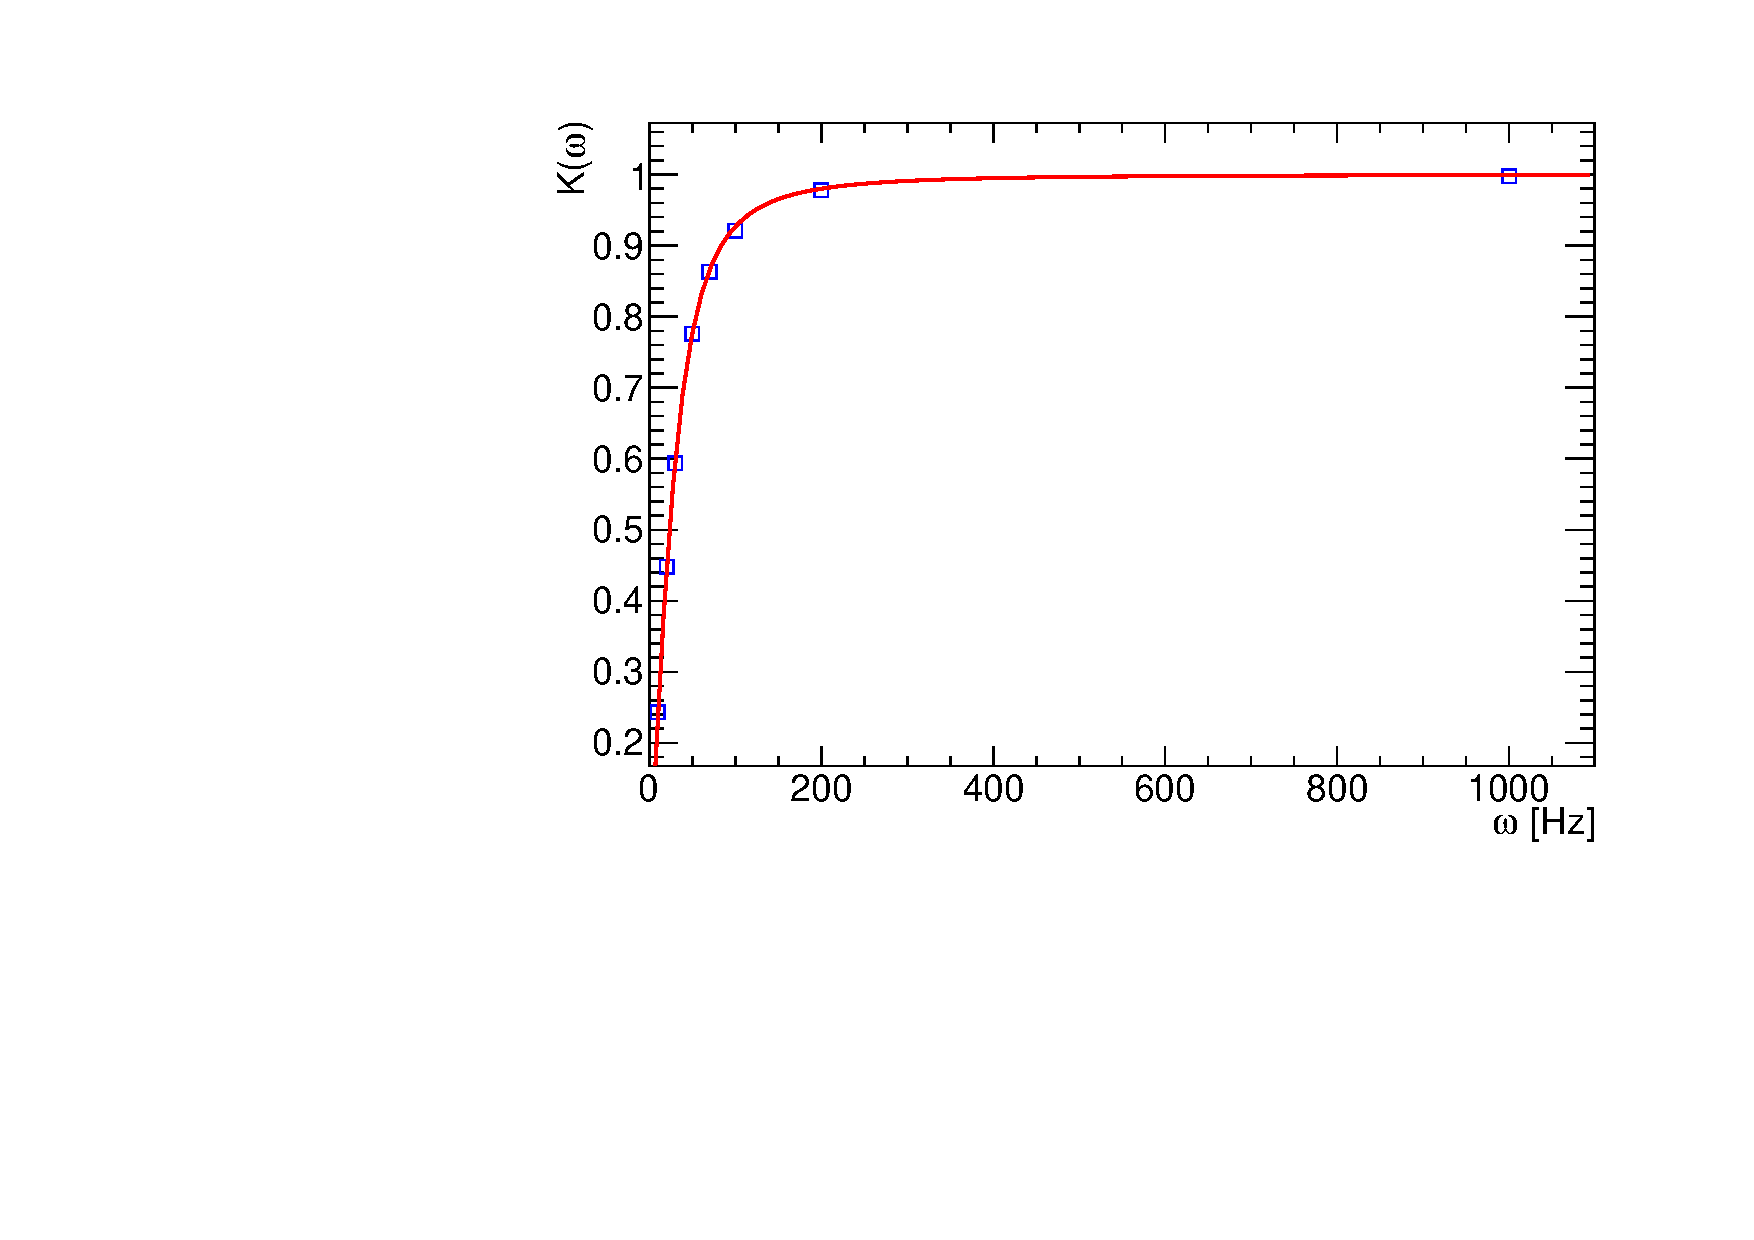
\includegraphics[width=1\linewidth]{sind/k.pdf}} \\$K(\omega)$ для диферинціюйочого чотирьохполюсника
	\end{minipage}
	\hfill
	\begin{minipage}[h]{0.4\linewidth}
		\center{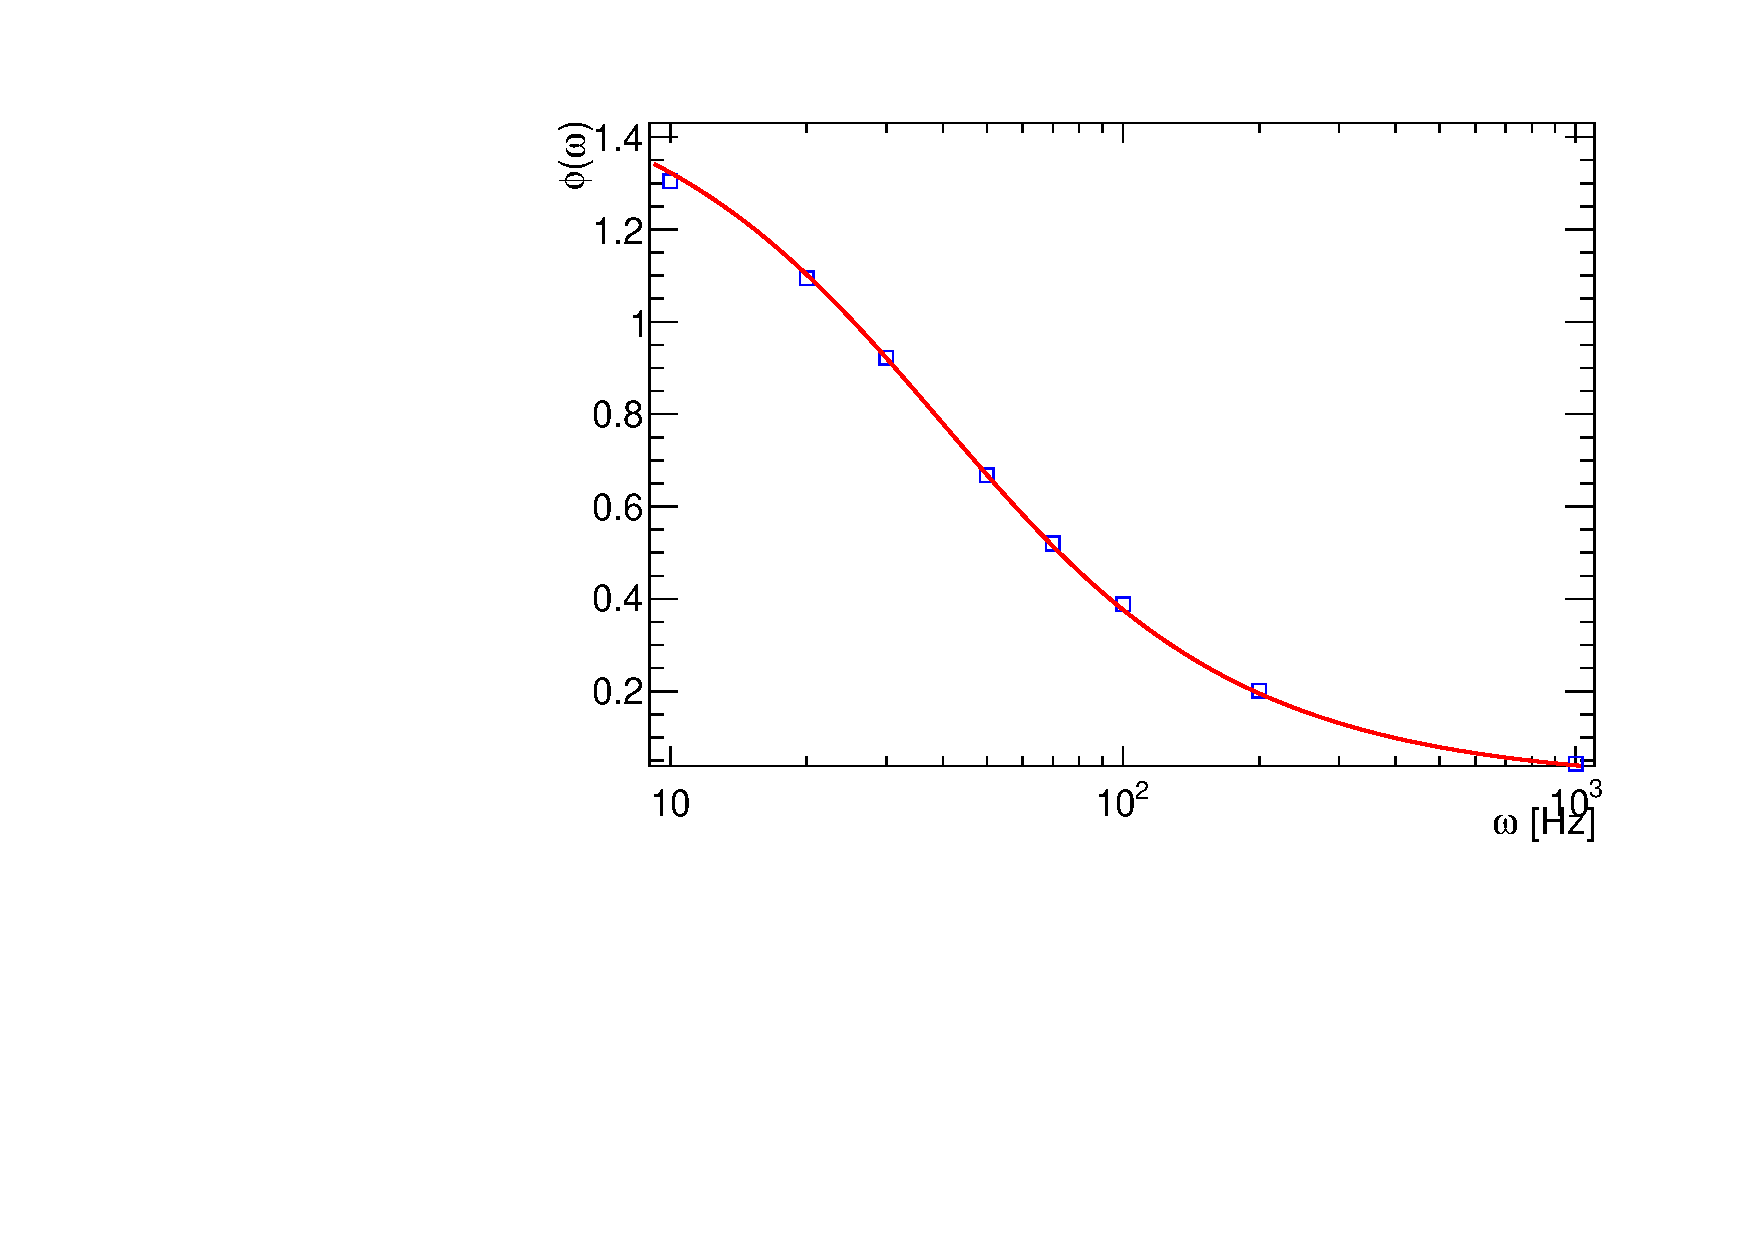
\includegraphics[width=1\linewidth]{sind/phi.pdf}} \\$\phi(\omega)$ для диферинціюйочого чотирьохполюсника
	\end{minipage}
	\vfill
	\begin{minipage}[h]{0.4\linewidth}
		\center{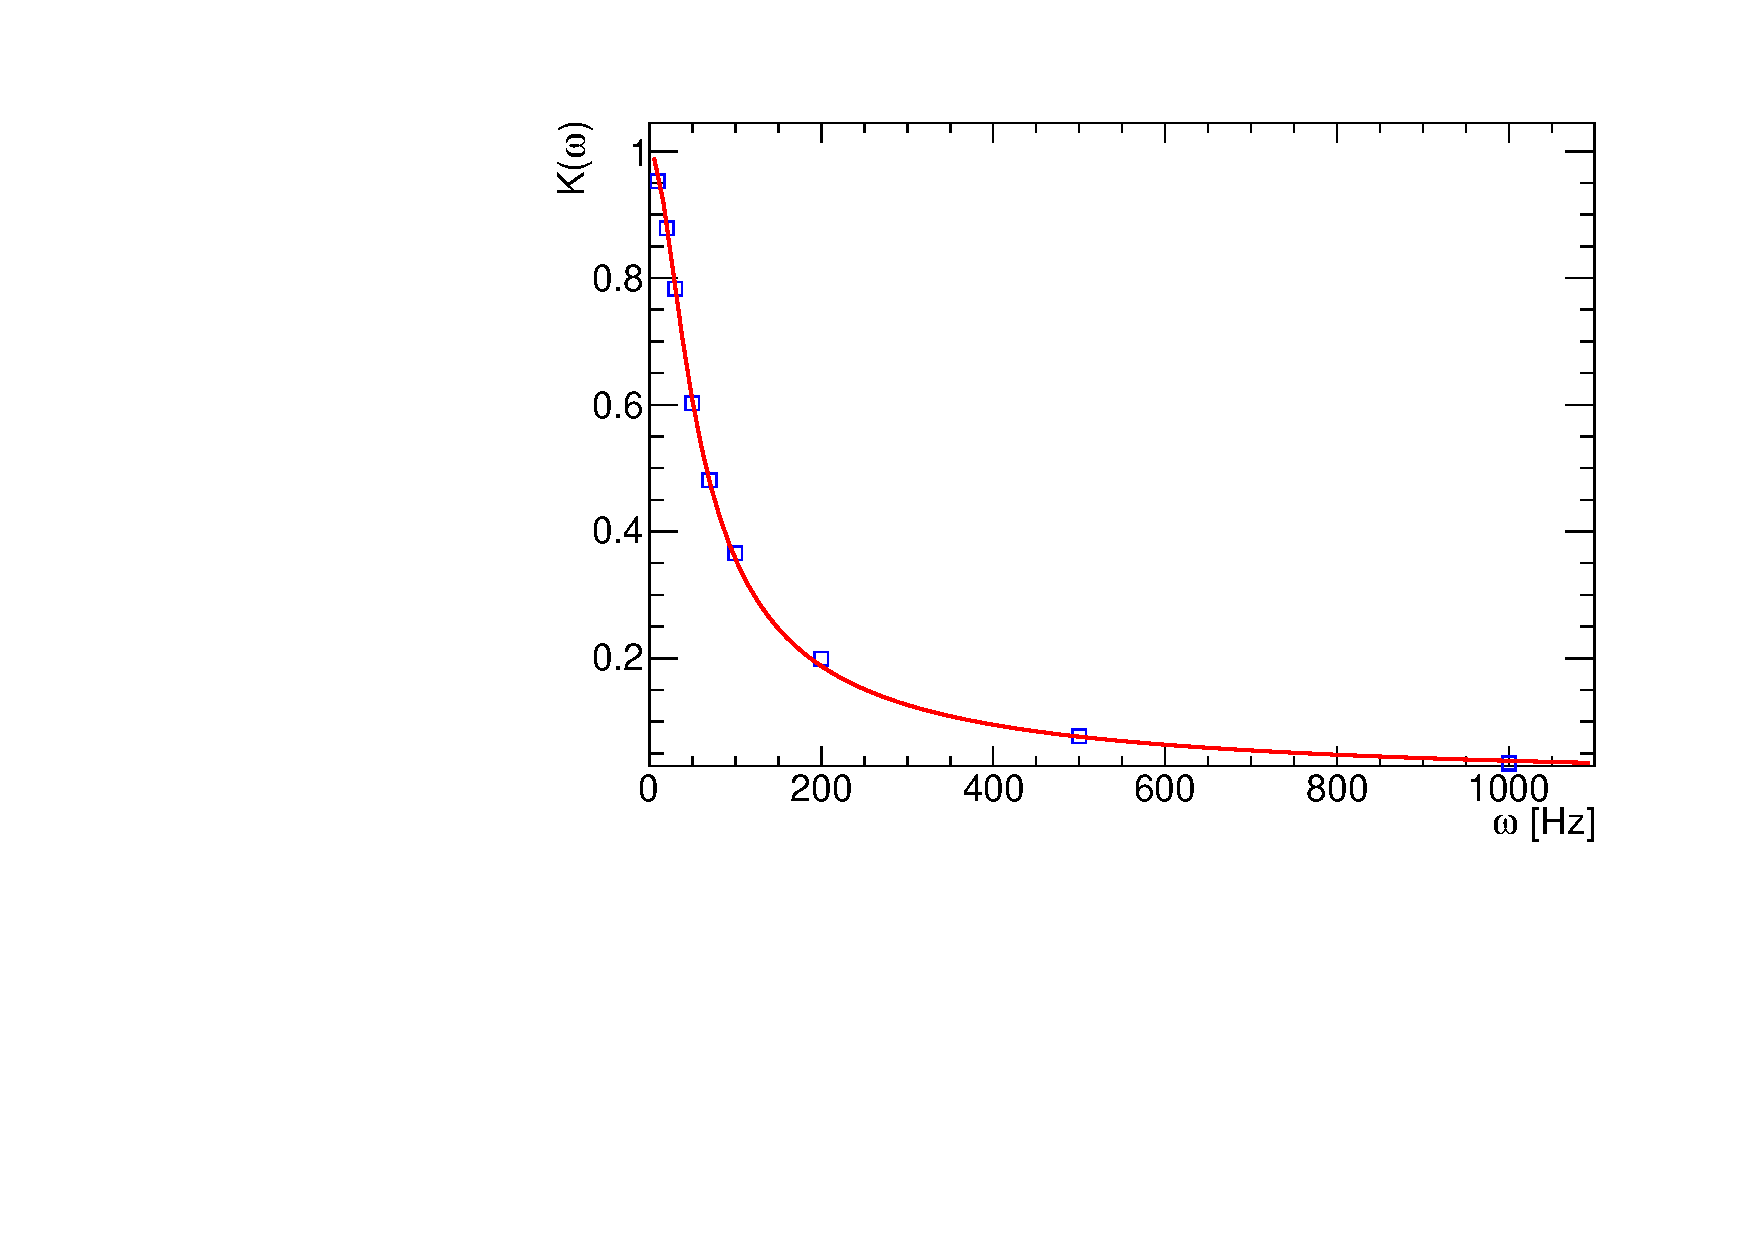
\includegraphics[width=1\linewidth]{sini/k.pdf}} \\$K(\omega)$ для інтегруючого чотирьохполюсника
	\end{minipage}
	\hfill
	\begin{minipage}[h]{0.4\linewidth}
		\center{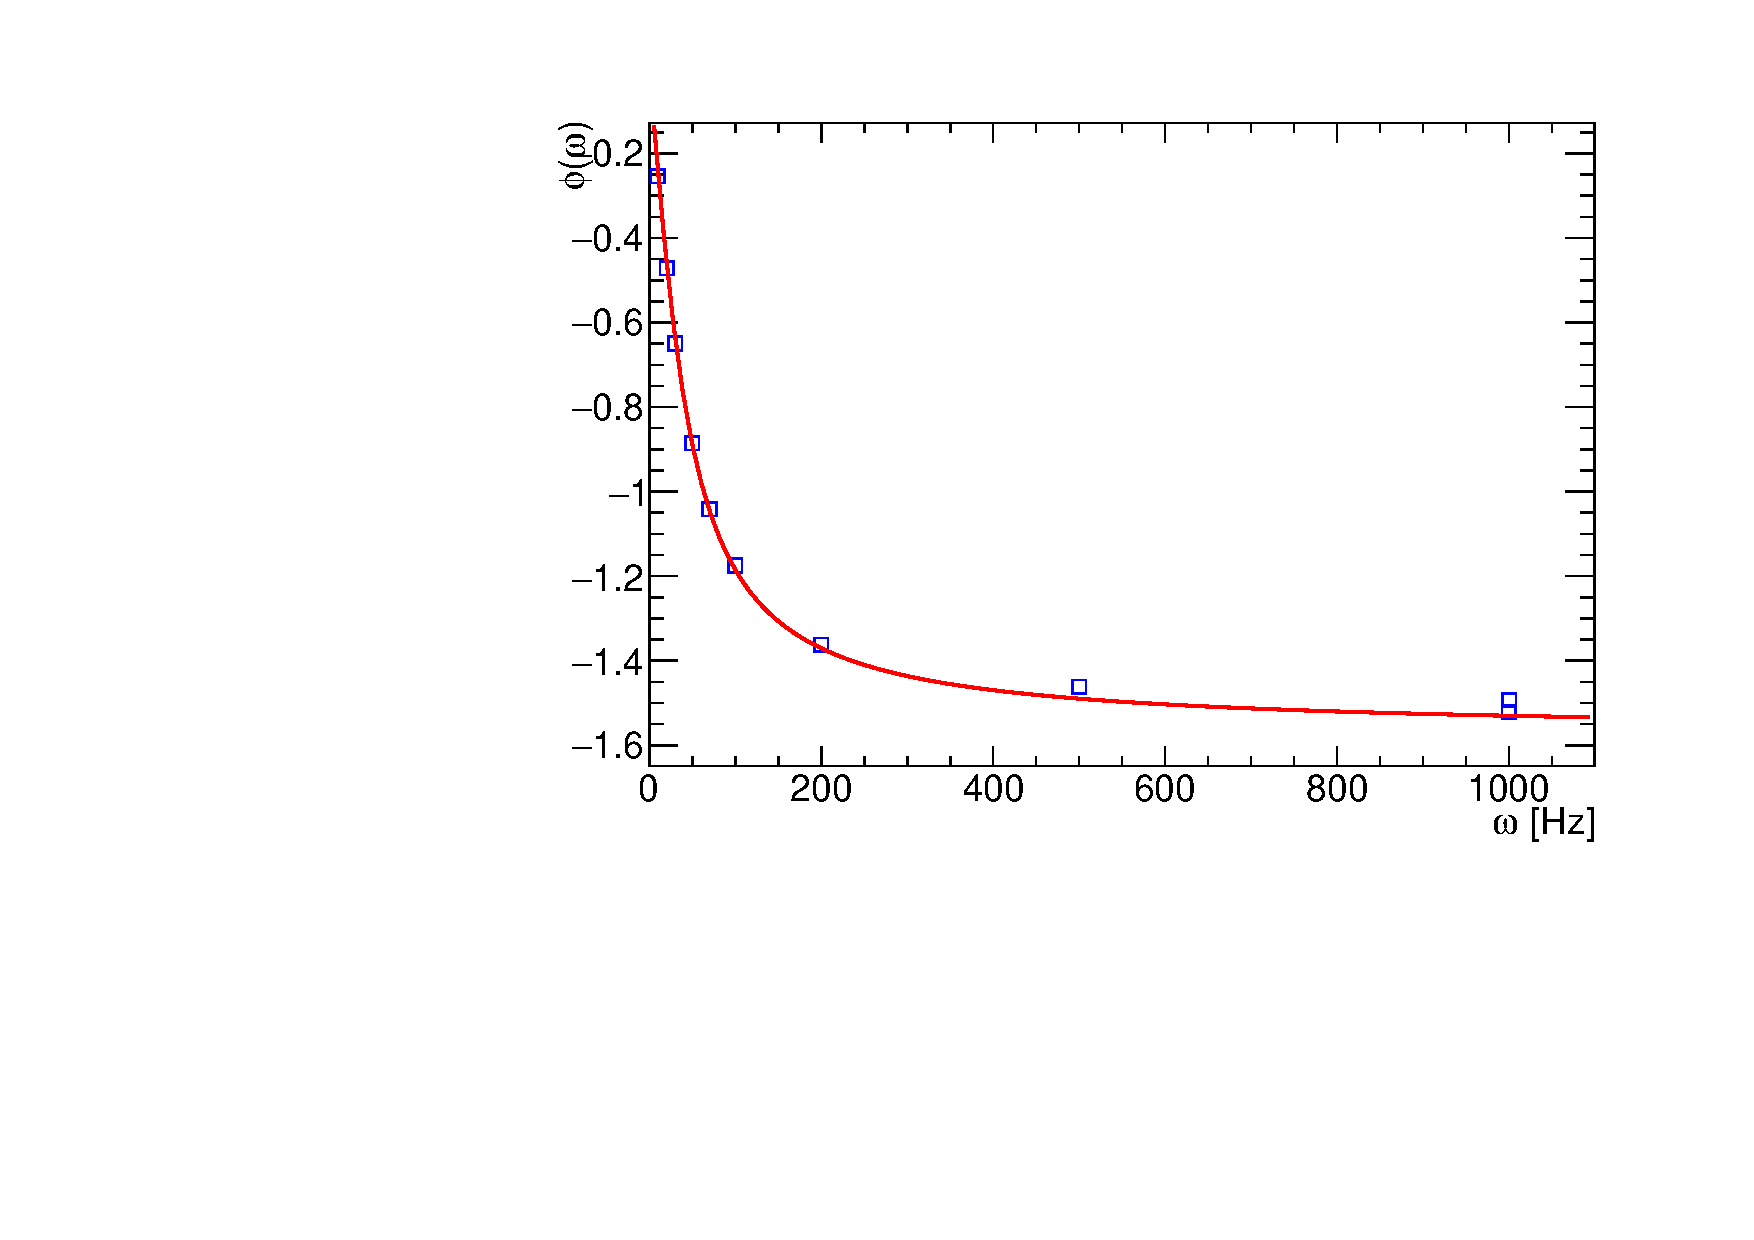
\includegraphics[width=1\linewidth]{sini/phi.pdf}} \\$\phi(\omega)$ для інтегруючого чотирьохполюсника
	\end{minipage}
	\caption{Отримані залежності відношення амплітуд $K(\omega)$ та зсуву фаз $\phi(\omega)$. Було апроксимано відповідно до моделей \ref{theoryD} та \ref{theoryI}}
	\label{fig:expkph}
\end{figure}
